\documentclass[a4paper,14pt]{extarticle}

\usepackage{fontspec}
\usepackage{polyglossia}
\setmainlanguage{russian}
\setmainfont{Times New Roman}
\setmonofont{Consolas}

\usepackage{geometry}
\geometry{left=2.5cm,right=1.5cm,top=2cm,bottom=2cm}
\usepackage{setspace}
\onehalfspacing
\usepackage{graphicx}
\usepackage{float}
\usepackage{caption}
\usepackage{enumitem}
\usepackage{booktabs}
\usepackage{longtable}
\usepackage{array}
\usepackage{hyperref}
\usepackage{fvextra}
\usepackage{xcolor}

\setlist{nosep,leftmargin=1.5em}
\captionsetup{font=small,skip=6pt}
\hypersetup{
  colorlinks=true,
  linkcolor=black,
  urlcolor=blue,
  pdftitle={Лабораторная работа 1. Автоматизация ввода ФИО}
}
\fvset{baselinestretch=0.9,commandchars=none}
\RecustomVerbatimEnvironment{Verbatim}{Verbatim}{breaklines,breakanywhere,fontsize=\scriptsize}

\begin{document}

\begin{titlepage}
\centering
Министерство науки и высшего образования Российской Федерации\\[6pt]
\underline{\hspace{0.86\textwidth}}\\
(наименование образовательной организации)\\[18pt]
\underline{\hspace{0.86\textwidth}}\\
(наименование кафедры)\\[48pt]
{\Large Лабораторная работа №\,1}\\[10pt]
по дисциплине\\
«Технологии промышленной разработки программного обеспечения.\\
Основные понятия»\\[18pt]
{\large Автоматизация ввода списка ФИО\\
редактированием «на лету»}\\[56pt]
\begin{flushleft}
\hspace{0.42\textwidth}
\begin{tabular}{ll}
Выполнил: & студент группы \underline{\hspace{2.2cm}}\\[8pt]
& \underline{\hspace{5.2cm}}\\
& (ФИО)\\[16pt]
Проверил: & \underline{\hspace{5.2cm}}\\
& (ФИО, должность)\\
\end{tabular}
\end{flushleft}
\vfill
\underline{\hspace{4cm}} --- 2026
\end{titlepage}

\tableofcontents
\newpage

\section{Описание работы}

\subsection{Цель и постановка}

Цель работы --- разработать типовое решение для автоматизации ввода списка значений редактированием «на лету»: обработчики клавиатуры приводят набираемый текст к заданному образцу, не требуя от оператора следить за регистром и знаками препинания.

По методическим указаниям образец обеспечивает формат ФИО: фамилия с прописной первой буквы и строчными остальными, один пробел, два инициала прописными буквами, после каждого инициала точка. Точки оператор не ставит. После второго инициала строка выделяется целиком, каретка остаётся справа. Если запись верна, следующий ввод убирает её из поля (в работе --- в список) и начинает новую строку. Если буква неверна, выделение снимается и текст исправляется.

Минимальная доработка образца --- двойная фамилия через дефис, например «Новиков-Прибой А.С.». Дополнительно требуется кодирование шаблона строки и режим, в котором первая строка задаёт шаблон, а следующие вводятся по нему.

\subsection{Недостатки базового образца}

Базовый обработчик \texttt{KeyPress} пропускает только буквы и пробел. Дефис попадает в ветку \texttt{e.Handled = true} и не вводится. Ветвь для букв фамилии после первой пустая, поэтому регистр хвоста фамилии не приводится к строчным. Счётчик \texttt{space} увеличивается только вперёд и расходится с текстом после \texttt{Backspace}. Сам \texttt{Backspace} не является буквой и тоже блокируется. Универсального шаблона в образце нет.

\subsection{Принятое решение}

Логика ввода вынесена из формы в ядро, которое не зависит от Windows Forms. Форма только передаёт символы и показывает состояние.

Шаблон --- это строка из латинских кодов. Смысл кодов:

\begin{center}
\begin{tabular}{lll}
\toprule
Код & Смысл & В строке результата\\
\midrule
\texttt{W} & слово произвольной длины & первая буква прописная, остальные строчные\\
\texttt{I} & инициал & одна прописная буква и точка\\
\texttt{-} & дефис & символ «-»\\
пробел & один разделитель & один пробел\\
\texttt{.} & оформление шаблона & в результат не входит\\
\texttt{[-W]} & необязательная группа & дефис и ещё одно слово, либо пропуск\\
\bottomrule
\end{tabular}
\end{center}

Если слово в шаблоне записано сразу перед инициалом (\texttt{WII}, \texttt{W-WII}), между ними автоматически добавляется пробел. Необязательная группа обязана начинаться с разделителя: буква после буквы не позволяет понять, где кончилось слово.

Шаблон по умолчанию --- \texttt{W[-W][-W] II}. Он покрывает минимальное требование и обычный ввод без дефиса:

\begin{center}
\begin{tabular}{ll}
\toprule
Нажатия оператора & Результат\\
\midrule
\texttt{иванов ас} & Иванов А.С.\\
\texttt{новиков-прибой ас} & Новиков-Прибой А.С.\\
\texttt{алёшин-боров-волков ис} & Алёшин-Боров-Волков И.С.\\
\bottomrule
\end{tabular}
\end{center}

Четвёртая часть фамилии по этому шаблону не принимается: необязательных групп две.

Первая строка поля --- шаблон, если её набирают кодами и подтверждают клавишей Enter. Кириллическая буква с пустой строки сразу включает шаблон по умолчанию, поэтому оператор может начать список, не изучая коды. Пустой Enter делает то же самое. Клавиша F2 открывает ввод нового шаблона, уже накопленный список не стирается.

Готовая строка, в которую больше нельзя добавить символ, выделяется целиком. Каретка ставится справа сообщением \texttt{EM\_SETSEL} с границами 0 и $-1$. Следующая буква переносит запись в список и начинает новую. Enter сохраняет готовую запись и очищает поле. \texttt{Backspace} удаляет последний символ, в том числе автоматически поставленную точку. Стрелка влево только снимает выделение.

Регистр считается по культуре \texttt{ru-RU}, поэтому «ё» переходит в «Ё», а не в «Е».

\section{Код}

Решение --- три проекта SDK-стиля на .NET 10:

\begin{itemize}
\item \texttt{Lab1Fio.Core} --- шаблон и сеанс ввода, без интерфейса;
\item \texttt{Lab1Fio.App} --- окно Windows Forms;
\item \texttt{Lab1Fio.Tests} --- модульные тесты xUnit.
\end{itemize}

Файл решения: \texttt{Lab1/Lab1.slnx}.

\subsection{Разбор шаблона}
\VerbatimInput[breaklines,breakanywhere,fontsize=\scriptsize,frame=single]{../Lab1/Lab1Fio.Core/TemplatePattern.cs}

\subsection{Сеанс ввода}
\VerbatimInput[breaklines,breakanywhere,fontsize=\scriptsize,frame=single]{../Lab1/Lab1Fio.Core/FioSession.cs}

\subsection{Окно}
\VerbatimInput[breaklines,breakanywhere,fontsize=\scriptsize,frame=single]{../Lab1/Lab1Fio.App/Program.cs}
\VerbatimInput[breaklines,breakanywhere,fontsize=\scriptsize,frame=single]{../Lab1/Lab1Fio.App/MainForm.cs}

\subsection{Модульные тесты}
\VerbatimInput[breaklines,breakanywhere,fontsize=\scriptsize,frame=single]{../Lab1/Lab1Fio.Tests/FioInputTests.cs}

\section{Описание написанного кода}

\subsection{TemplatePattern}

Класс хранит шаблон двумя представлениями. Список элементов нужен для канонической записи, маски \texttt{Ааа[-Ааа] А.А.} и примера. Список шагов нужен для разбора уже набранного текста: обязательный атом (\texttt{W}, \texttt{-}, пробел, \texttt{I}) --- отдельный шаг, группа в скобках --- один необязательный шаг из нескольких атомов.

\texttt{TryParse} читает строку, пропускает точки, схлопывает повторные пробелы, отвергает неизвестные символы, пустые и вложенные скобки. Затем вставляет пробел между словом и инициалом и проверяет соседей. Два слова подряд, дефис без следующего \texttt{W}, шаблон, который начинается или кончается разделителем, --- ошибка с текстом на русском языке.

\texttt{Evaluate} отвечает на вопрос, чем можно продолжить уже набранный префикс. Обход идёт по шагам и по тексту. Слово забирает всю непрерывную цепочку букв: граница слова --- не буква, поэтому развилка «где кончилась фамилия» не нужна. Необязательный шаг либо берётся, если следующий символ ему подходит, либо пропускается. На конце текста метод собирает множество действий: первая буква слова, продолжение слова строчной, дефис, пробел, буква инициала, точка, завершение.

Запись считается законченной и блокируется, только если допустимо единственное действие --- завершение. Тогда форма выделяет текст. Если одновременно можно и дописать букву, и нажать Enter (шаблон из одного \texttt{W}), строка сохраняется по Enter, но не выделяется: иначе следующая буква начала бы новую запись вместо продолжения слова.

\subsection{FioSession}

Сеанс --- единственный владелец текста, списка и режима. Форма после каждого нажатия перерисовывает поле из свойств сеанса и ставит \texttt{e.Handled = true}, поэтому в \texttt{TextBox} не попадает символ, который сеанс отклонил.

В режиме шаблона принимаются \texttt{W}, \texttt{I}, дефис, пробел, точка и скобки. Буквы \texttt{w} и \texttt{i} поднимаются к верхнему регистру. Любая другая буква при пустом поле включает шаблон по умолчанию и тут же обрабатывается как первая буква ФИО. Если коды шаблона уже набраны, кириллица отклоняется, чтобы не смешать два режима.

В режиме данных символ сверяется с \texttt{MatchState}. Буква инициала сразу дополняется точкой. Если точку стёрли и следом идёт ещё один инициал, буква вставляет недостающую точку, новую букву и её точку. Завершённая строка при следующей букве сначала попадает в список, затем эта буква начинает новую запись. Цифра, лишний пробел и дефис там, где шаблон его не ждёт, текст не меняют: в статусе остаётся подсказка, что можно ввести.

\texttt{Backspace} удаляет ровно один символ и заново вычисляет выделение. Счётчик, как в образце, не используется, поэтому правка с конца строки не ломает автомат.

\subsection{MainForm}

Окно показывает памятку по кодам, строку активного шаблона и маски, поле ввода, статус и список. Жёлтый фон поля --- режим шаблона, зелёный --- готовая запись, красный статус --- отказ. \texttt{EM\_SETSEL(0, -1)} выделяет весь текст и оставляет каретку справа, как требует методичка: обычные \texttt{SelectionStart} и \texttt{SelectionLength} ставят каретку в начало выделения.

Клавиши: Enter --- подтвердить шаблон или сохранить запись; Backspace и Delete --- стереть последний символ; стрелки --- снять выделение; Escape --- отменить набор нового шаблона; F2 --- новый шаблон; Ctrl+V --- вставить текст посимвольно через тот же фильтр.

\section{Описание тестовых сценариев}

Проверяются два слоя.

Ядро проверяется без окна: 34 теста xUnit вызывают \texttt{FioSession} и \texttt{TemplatePattern} так же, как форма вызывает их на \texttt{KeyPress}. Тест набирает строку посимвольно, включая заведомо «грязный» регистр. Так видно и отказ символа, и итоговый текст, и состав списка, и флаг выделения. Команда:

\begin{Verbatim}
dotnet test Lab1/Lab1.slnx
\end{Verbatim}

Результат прогона: не пройдено 0, пройдено 34.

Окно проверяется отдельным запуском с аргументом \texttt{--demo-out}. Форма сама выполняет те же сценарии и сохраняет снимок после каждого контрольного состояния. Снимки лежат в \texttt{report/images} и приведены в следующем разделе. Снимок фиксирует то, что видит оператор: подсказку, цвет поля, выделение и список.

Группы сценариев:

\begin{enumerate}
\item разбор шаблона: канонический вид, точки в записи шаблона, автопробел, отказ пустой строки, двойного дефиса, \texttt{WW}, скобок без разделителя;
\item шаблон по умолчанию: одна, две и три части фамилии, отказ четвёртой части, регистр, буква «ё»;
\item запреты: цифра, пробел в начале, второй пробел подряд, пробел вместо обязательного дефиса;
\item завершение: выделение, Enter, следующая буква уносит запись в список, незавершённый Enter запись не создаёт;
\item правка: стереть неверный инициал и ввести верный; восстановить стёртую точку перед следующим инициалом;
\item смена шаблона: \texttt{W I I} даёт пробел между инициалами, список прежних записей сохраняется;
\item шаблон из одного слова сохраняется по Enter и при этом принимает ещё буквы.
\end{enumerate}

\section{Тестовые сценарии}

Ниже --- сценарии, выполненные в окне. Ожидаемый текст совпал с фактическим. Модульные тесты проверяют те же строки программно.

\subsection{Старт: первая строка --- шаблон}

Шаги: запустить приложение.\\
Ожидание: поле пустое, фон жёлтый, подсказка предлагает шаблон или кириллицу, список пуст.\\
Факт: совпало, рисунок~\ref{fig:start}.

\begin{figure}[H]
\centering
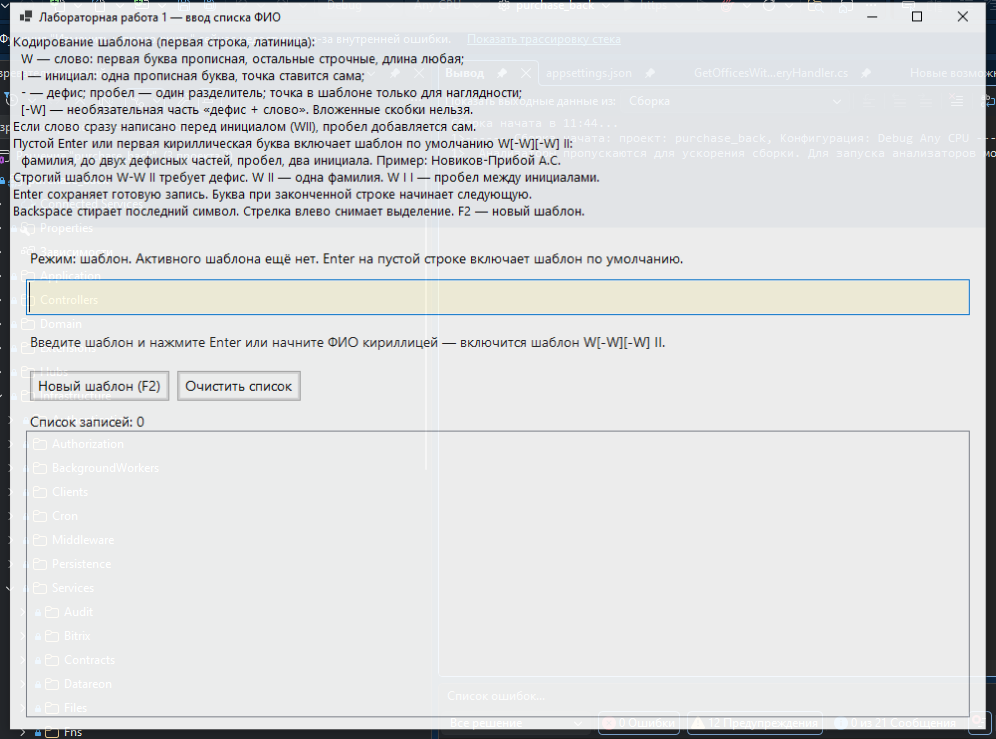
\includegraphics[width=\textwidth]{images/01-start.png}
\caption{Режим шаблона при запуске}
\label{fig:start}
\end{figure}

\subsection{Двойная фамилия без предварительной настройки}

Шаги: с пустого поля набрать \texttt{новиков-прибой ас} без точек и без заботы о регистре.\\
Ожидание: шаблон по умолчанию \texttt{W[-W][-W] II}, текст «Новиков-Прибой А.С.», поле зелёное, строка выделена.\\
Факт: совпало, рисунок~\ref{fig:double}.

\begin{figure}[H]
\centering
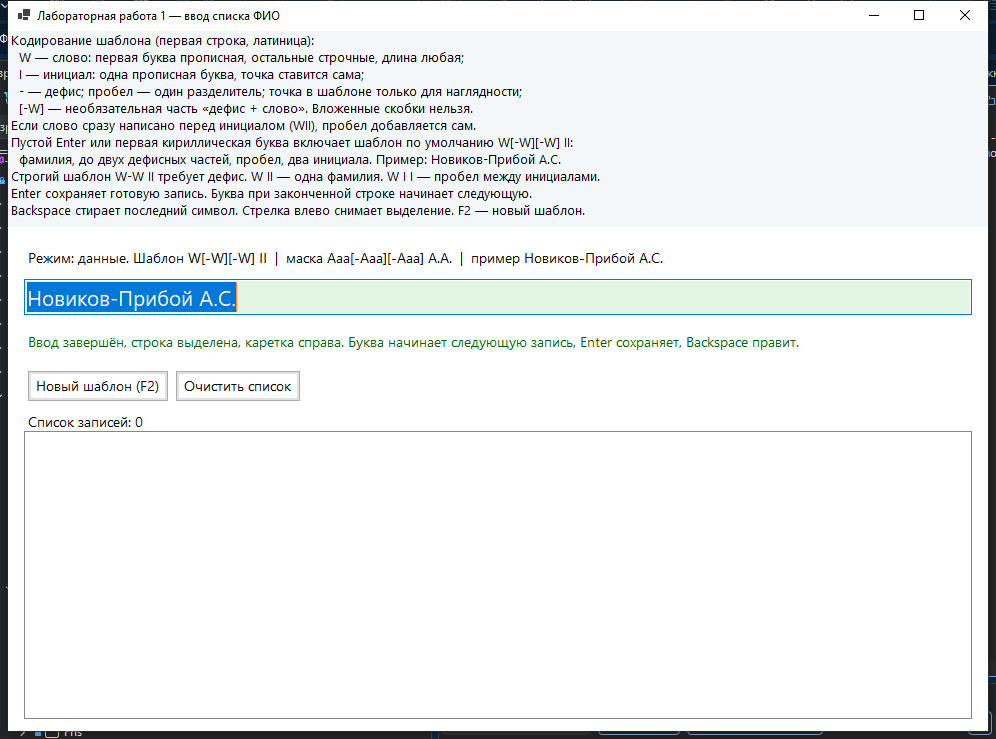
\includegraphics[width=\textwidth]{images/02-double-complete.png}
\caption{Готовая запись «Новиков-Прибой А.С.»}
\label{fig:double}
\end{figure}

\subsection{Список из разных форм фамилии}

Шаги: Enter после двойной фамилии; набрать \texttt{иванов ас}, Enter; набрать \texttt{мамин-сибиряк дн}, Enter.\\
Ожидание: в списке три строки --- «Новиков-Прибой А.С.», «Иванов А.С.», «Мамин-Сибиряк Д.Н.», поле пустое.\\
Факт: совпало, рисунок~\ref{fig:list}.

\begin{figure}[H]
\centering
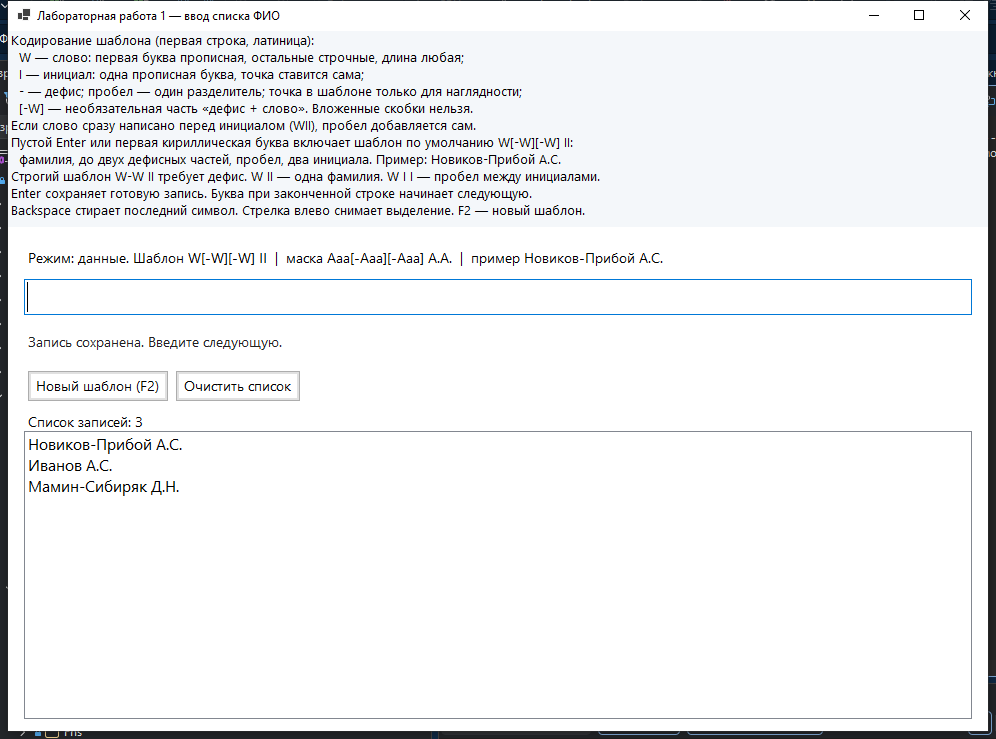
\includegraphics[width=\textwidth]{images/03-list.png}
\caption{Список после трёх записей}
\label{fig:list}
\end{figure}

\subsection{Отказ цифры}

Шаги: при пустом поле данных нажать \texttt{7}.\\
Ожидание: поле остаётся пустым, статус красный, список не меняется.\\
Факт: совпало, рисунок~\ref{fig:digit}.

\begin{figure}[H]
\centering
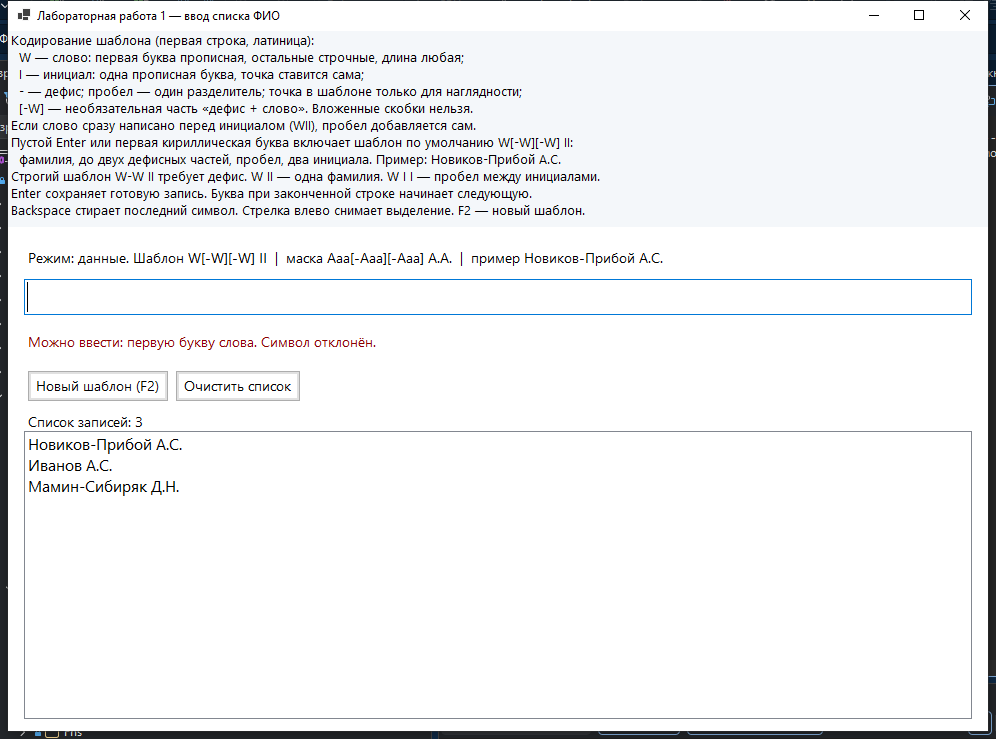
\includegraphics[width=\textwidth]{images/04-reject-digit.png}
\caption{Цифра отклонена, список цел}
\label{fig:digit}
\end{figure}

\subsection{Фамилия из трёх частей}

Шаги: набрать \texttt{алёшин-боров-волков ис}.\\
Ожидание: «Алёшин-Боров-Волков И.С.», буква «ё» сохранена.\\
Факт: совпало, рисунок~\ref{fig:triple}.

\begin{figure}[H]
\centering
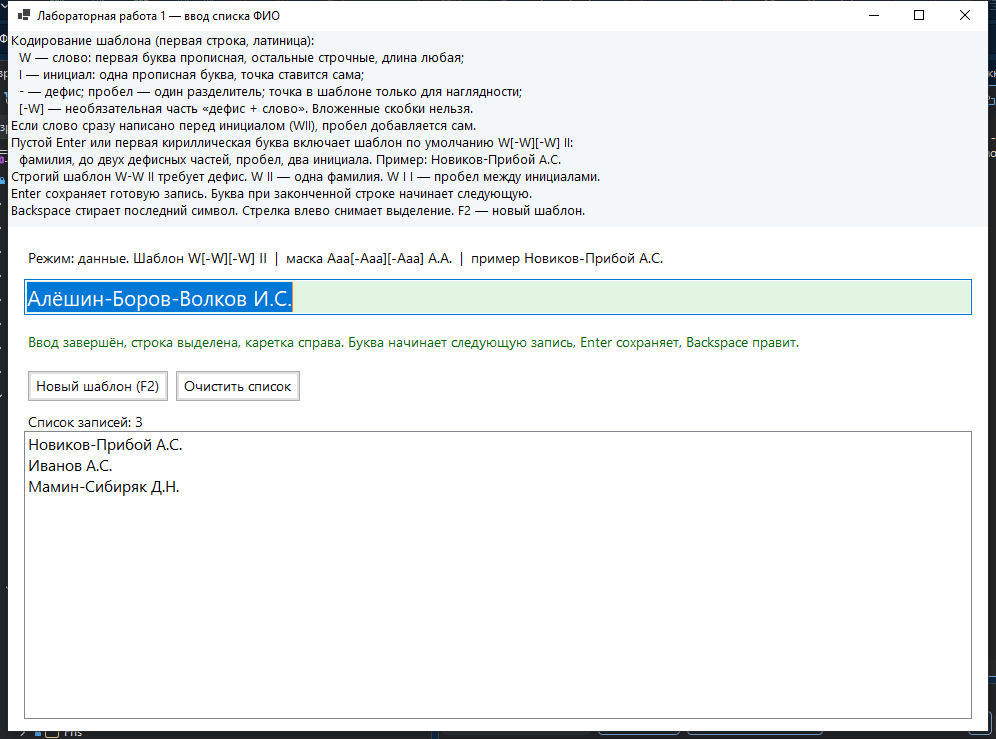
\includegraphics[width=\textwidth]{images/05-triple.png}
\caption{Три части фамилии по шаблону по умолчанию}
\label{fig:triple}
\end{figure}

\subsection{Неверный инициал и исправление}

Шаги: набрать \texttt{иванов аы}. Убедиться, что получилось «Иванов А.Ы.». Снять выделение стрелкой влево, два раза \texttt{Backspace}, набрать \texttt{с}.\\
Ожидание: «Иванов А.С.», строка снова выделена.\\
Факт: до правки --- рисунок~\ref{fig:wrong}, после правки --- рисунок~\ref{fig:fixed}.

\begin{figure}[H]
\centering
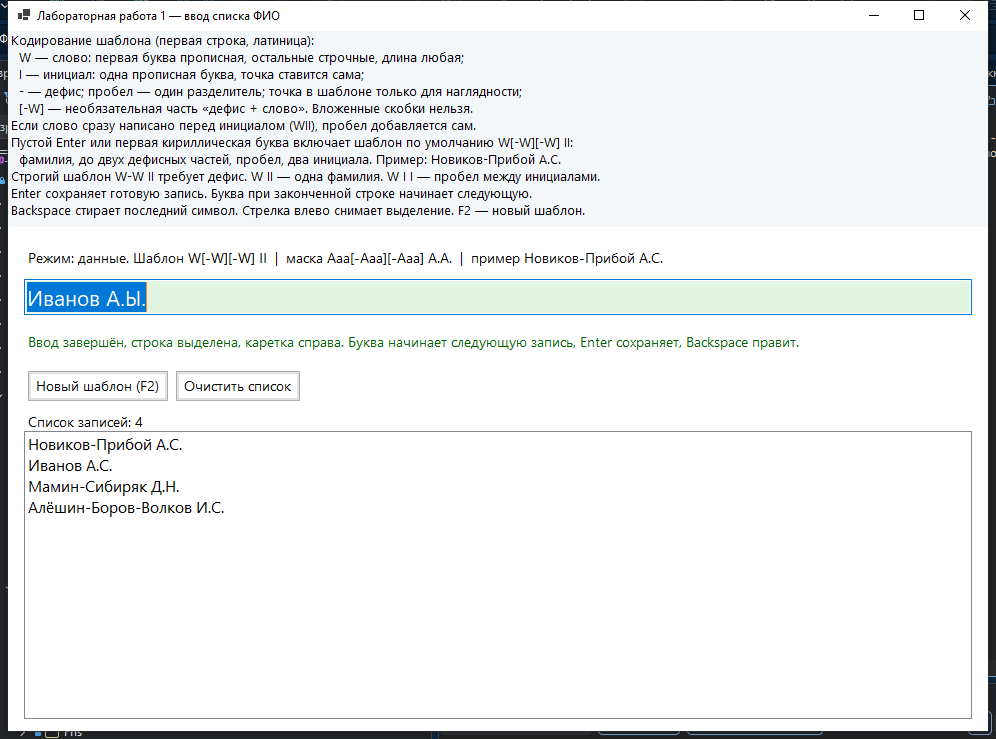
\includegraphics[width=\textwidth]{images/06-wrong-initial.png}
\caption{Ошибочный второй инициал «Ы»}
\label{fig:wrong}
\end{figure}

\begin{figure}[H]
\centering
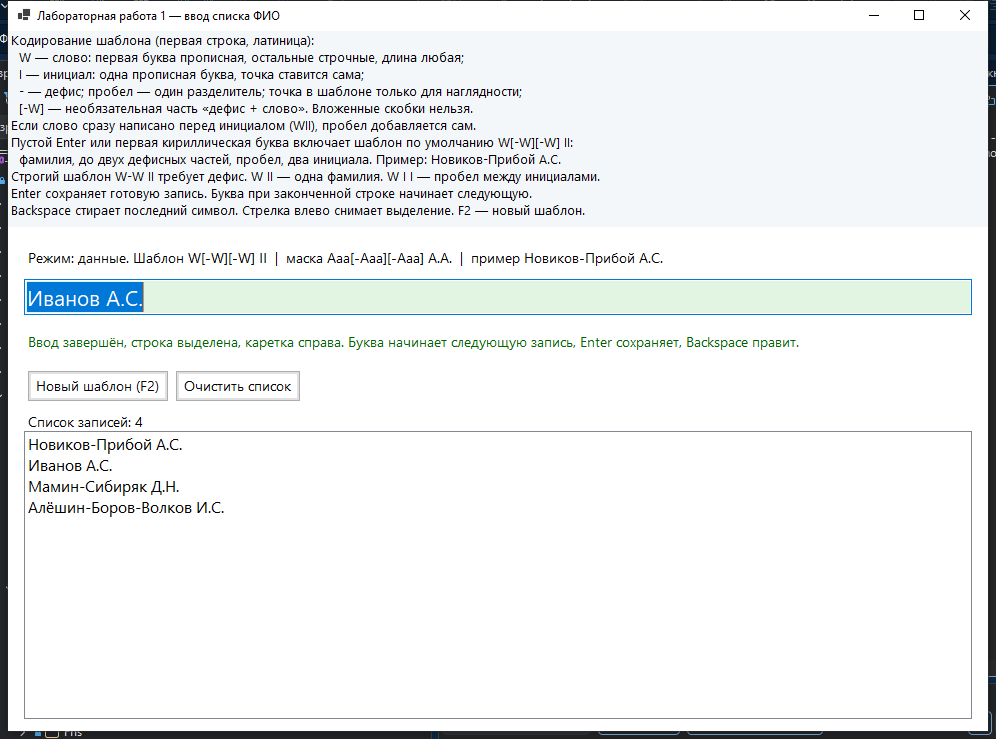
\includegraphics[width=\textwidth]{images/07-corrected.png}
\caption{После Backspace и буквы «с» --- «Иванов А.С.»}
\label{fig:fixed}
\end{figure}

\subsection{Первая строка задаёт строгий шаблон}

Шаги: F2, набрать \texttt{W-W II}.\\
Ожидание: жёлтое поле, статус предлагает принять шаблон, пример --- «Новиков-Прибой А.С.».\\
Факт: совпало, рисунок~\ref{fig:typed}.

\begin{figure}[H]
\centering
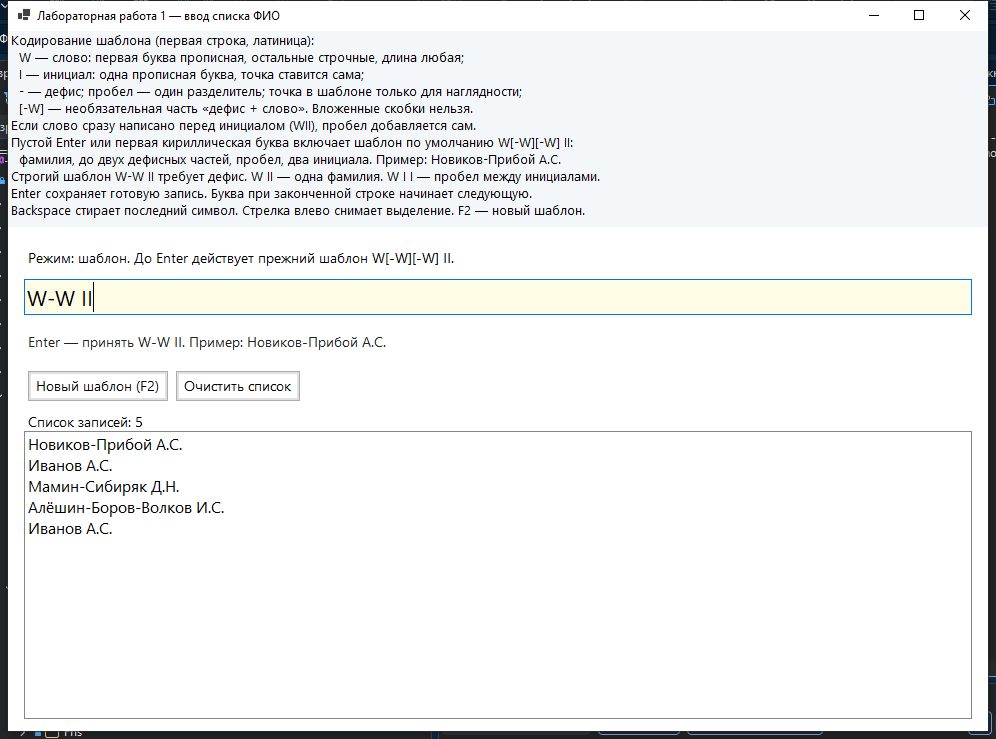
\includegraphics[width=\textwidth]{images/08-template-typed.png}
\caption{Набранный шаблон \texttt{W-W II} до Enter}
\label{fig:typed}
\end{figure}

Шаги: Enter.\\
Ожидание: режим данных, маска \texttt{Ааа-Ааа А.А.}, поле пустое, список прежний.\\
Факт: совпало, рисунок~\ref{fig:accepted}.

\begin{figure}[H]
\centering
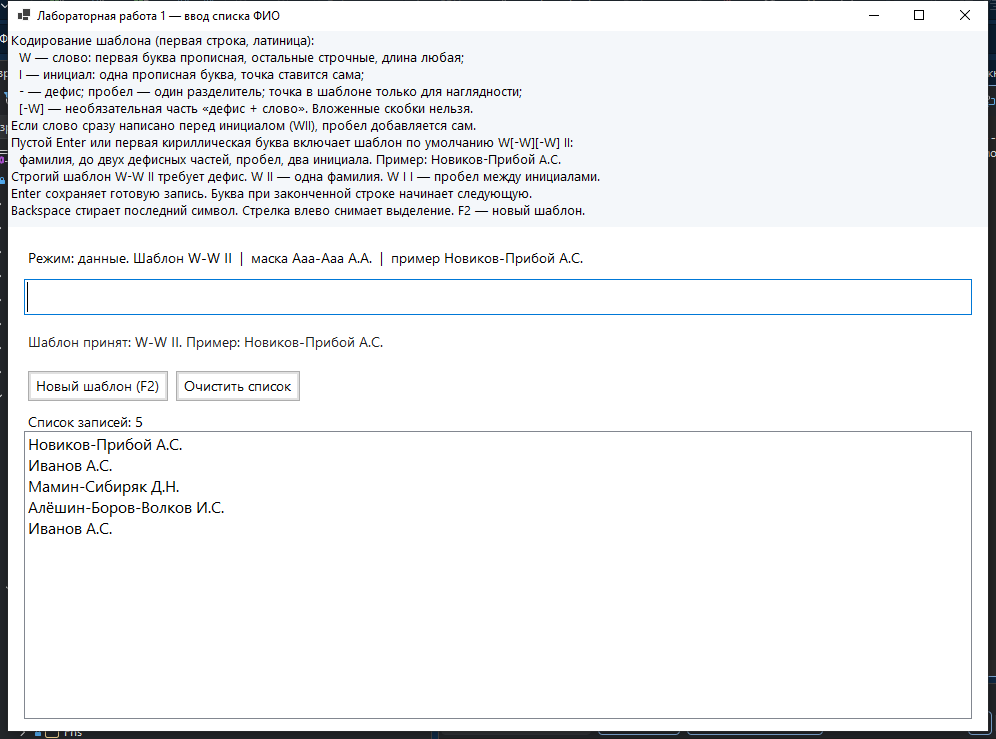
\includegraphics[width=\textwidth]{images/09-template-accepted.png}
\caption{Шаблон \texttt{W-W II} принят}
\label{fig:accepted}
\end{figure}

\subsection{Обязательный дефис}

Шаги: при шаблоне \texttt{W-W II} набрать \texttt{новиков} и пробел.\\
Ожидание: текст остаётся «Новиков», пробел отклонён, подсказка называет дефис.\\
Факт: совпало, рисунок~\ref{fig:hyphen}.

\begin{figure}[H]
\centering
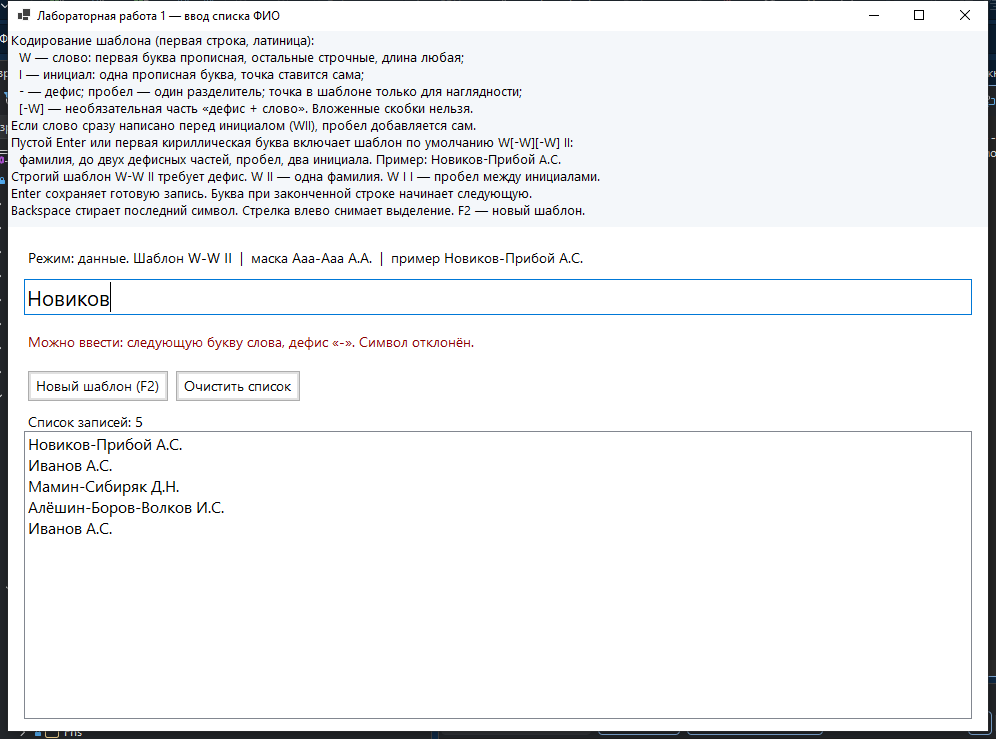
\includegraphics[width=\textwidth]{images/10-hyphen-required.png}
\caption{Пробел вместо дефиса отклонён}
\label{fig:hyphen}
\end{figure}

Шаги: набрать \texttt{-прибой ас}.\\
Ожидание: «Новиков-Прибой А.С.», строка выделена.\\
Факт: совпало, рисунок~\ref{fig:strict}.

\begin{figure}[H]
\centering
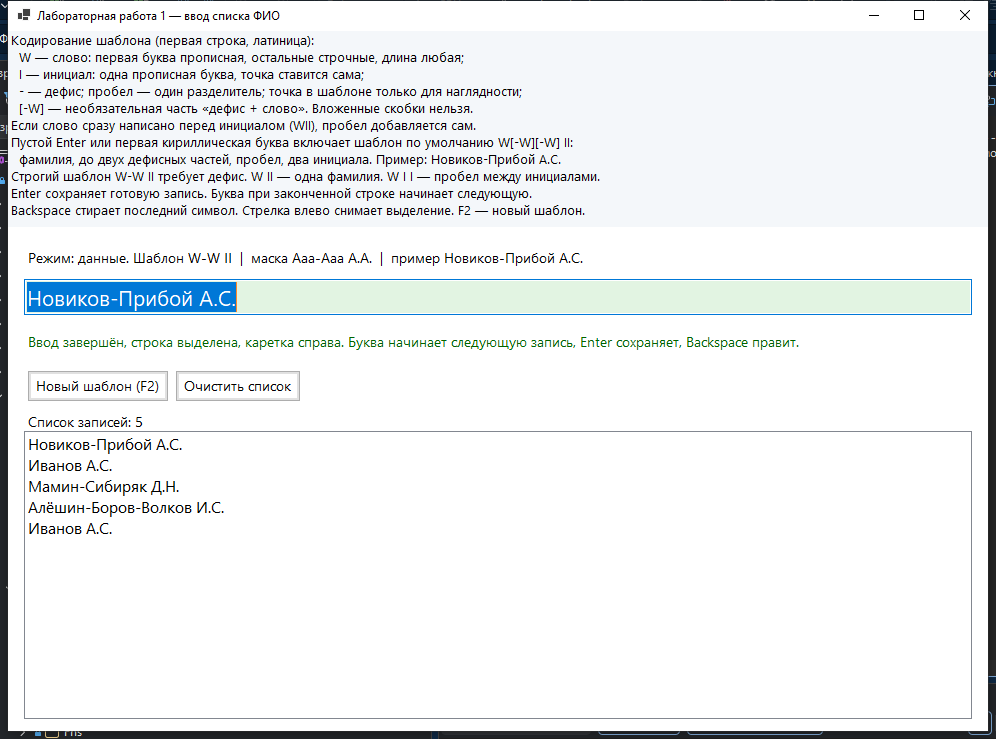
\includegraphics[width=\textwidth]{images/11-strict-complete.png}
\caption{Та же фамилия после обязательного дефиса}
\label{fig:strict}
\end{figure}

\subsection{Пробел между инициалами}

Шаги: F2, шаблон \texttt{W I I}, Enter, набрать \texttt{петров а с}.\\
Ожидание: «Петров А. С.» с пробелом между инициалами. Ранее сохранённые строки на месте.\\
Факт: совпало, рисунок~\ref{fig:space}.

\begin{figure}[H]
\centering
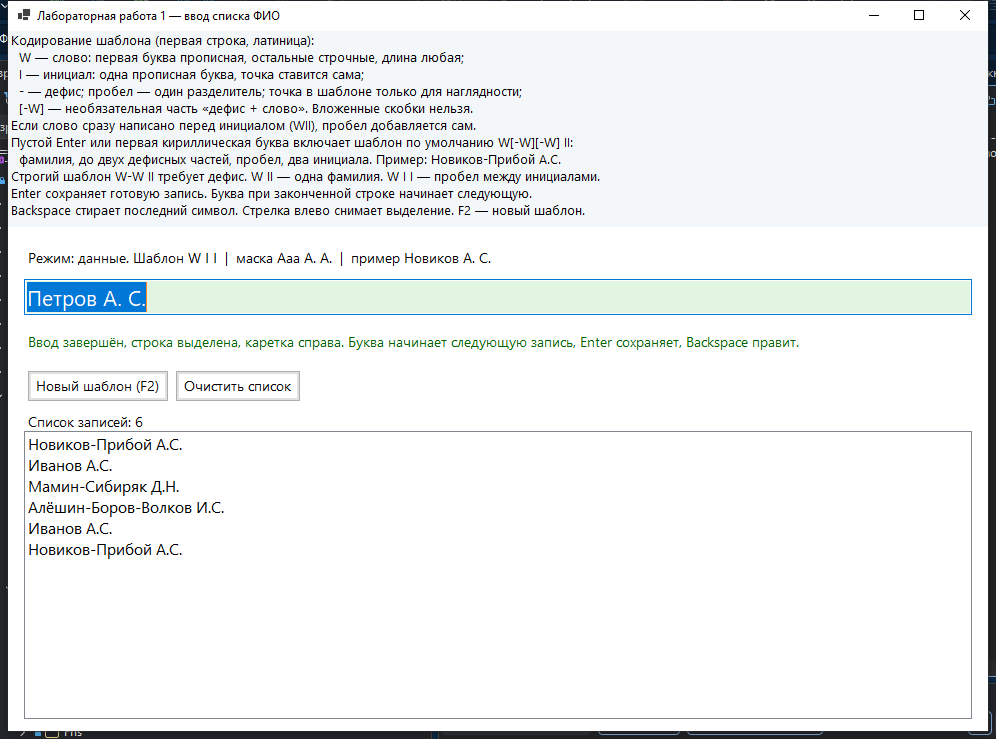
\includegraphics[width=\textwidth]{images/12-spaced-initials.png}
\caption{Шаблон \texttt{W I I}: «Петров А. С.»}
\label{fig:space}
\end{figure}

\subsection{Сценарии, закрытые только модульными тестами}

\begin{center}
\begin{tabular}{p{0.34\textwidth}p{0.28\textwidth}p{0.28\textwidth}}
\toprule
Вход & Ожидание & Результат теста\\
\midrule
\texttt{НОВИКОВ-ПРИБОЙ АС} & Новиков-Прибой А.С. & пройден\\
\texttt{ёлкин-ёжиков} и два «ё» & Ёлкин-Ёжиков Ё.Ё. & пройден\\
четвёртый дефис после трёх частей & символ отклонён & пройден\\
Enter на слове «Иванов» без инициалов & список пуст & пройден\\
буква при выделенной готовой строке & строка в списке, в поле новая буква & пройден\\
шаблон \texttt{W}, затем ещё буква & слово растёт, Enter сохраняет & пройден\\
\texttt{W-WII}, \texttt{w-w ii}, \texttt{W-W I.I.} & канонический вид \texttt{W-W II} & пройден\\
пустой шаблон, \texttt{-W II}, \texttt{W--W II}, \texttt{WW}, \texttt{[W] II} & отказ разбора & пройден\\
\bottomrule
\end{tabular}
\end{center}

\section{Документация}

\subsection{Руководство оператора}

Запуск: \texttt{dotnet run --project Lab1/Lab1Fio.App}. Открывается одно окно.

Обычный список ФИО начинают сразу кириллицей либо нажимают Enter на пустом поле. Дальше фамилия набирается буквами, части двойной и тройной фамилии разделяются дефисом, после фамилии --- один пробел и две буквы инициалов. Точки появляются сами. Когда поле становится зелёным, запись готова: Enter кладёт её в список, либо первая буква следующей фамилии делает это сама.

Ошибку в конце строки исправляют так: стрелка влево снимает выделение, \texttt{Backspace} стирает символы с конца, нужные буквы набираются заново. Середину строки стрелками не правят: каретка удерживается в конце, чтобы фильтр шаблона не расходился с местом вставки.

Новый образец задают клавишей F2 или кнопкой «Новый шаблон». В жёлтом поле набирают коды и нажимают Enter. Escape возвращает прежний шаблон, если строка данных ещё не начата. Кнопка «Очистить список» удаляет только накопленные записи.

Вставка из буфера (Ctrl+V) проходит тем же фильтром, что и клавиши: лишние символы отбрасываются, регистр выправляется.

\subsection{Спецификация шаблона}

Алфавит: латинские \texttt{W} и \texttt{I} в любом регистре, дефис, пробел, точка, квадратные скобки. Остальные символы --- ошибка.

\begin{center}
\begin{tabular}{p{0.28\textwidth}p{0.62\textwidth}}
\toprule
Запись & Что получится\\
\midrule
\texttt{W II} & одна фамилия и два инициала: Иванов А.С.\\
\texttt{W-W II} & ровно одна дефисная фамилия\\
\texttt{W-W-W II} & ровно три части фамилии\\
\texttt{W[-W][-W] II} & одна, две или три части; это значение по умолчанию\\
\texttt{W I I} & пробел между инициалами: Иванов А. С.\\
\texttt{II} & только инициалы\\
\texttt{W} & одно слово, конец по Enter\\
\bottomrule
\end{tabular}
\end{center}

Точка после \texttt{I} в шаблоне необязательна: \texttt{I.I.} и \texttt{II} --- один и тот же шаблон. Повторные пробелы схлопываются. Группа \texttt{[-W]} пропускается, пока оператор не ввёл дефис. После дефиса слово уже обязательно. Вложенные скобки не поддерживаются. Группа не может начинаться с буквы.

Маска на экране --- схема результата: \texttt{Ааа} означает слово, \texttt{А.} --- инициал, квадратные скобки --- необязательную часть.

\subsection{Клавиши}

\begin{center}
\begin{tabular}{ll}
\toprule
Клавиша & Действие\\
\midrule
буквы, дефис, пробел & ввод, если символ сейчас допустим\\
Enter & принять шаблон или сохранить готовую запись\\
Backspace, Delete & удалить последний символ\\
стрелки, Home, End & снять выделение\\
Escape & отменить ввод нового шаблона\\
F2 & перейти к новому шаблону\\
Ctrl+V & вставить текст через фильтр\\
\bottomrule
\end{tabular}
\end{center}

\subsection{Сборка}

Нужен SDK .NET 10 с поддержкой Windows Forms. Из каталога \texttt{Lab1}:

\begin{Verbatim}
dotnet test Lab1.slnx
dotnet run --project Lab1Fio.App
\end{Verbatim}

Снимки сценариев повторно снимаются так:

\begin{Verbatim}
dotnet run --project Lab1Fio.App -- --demo-out=..\report\images
\end{Verbatim}

Отчёт собирается XeLaTeX из каталога \texttt{report} (нужны \texttt{polyglossia}, \texttt{fontspec}, \texttt{fvextra}):

\begin{Verbatim}
xelatex lab1_report.tex
xelatex lab1_report.tex
\end{Verbatim}

Второй проход нужен для оглавления.

\subsection{Ограничения}

Каретка не переносится в середину строки: исправление идёт с конца. Четвёртая дефисная часть требует своего шаблона, например \texttt{W-W-W-W II} или дополнительной группы \texttt{[-W]}. Латинская фамилия, которая начинается с \texttt{W} или \texttt{I}, с пустого поля будет понята как код шаблона; перед таким вводом нужно нажать Enter и тем самым зафиксировать шаблон данных. Шаблон не описывает произвольную пунктуацию, кроме дефиса, пробела и точки инициала.

\subsection{Состав поставки}

\begin{center}
\begin{tabular}{p{0.46\textwidth}p{0.46\textwidth}}
\toprule
Путь & Назначение\\
\midrule
\texttt{Lab1/Lab1.slnx} & решение\\
\texttt{Lab1/Lab1Fio.Core} & шаблон и сеанс\\
\texttt{Lab1/Lab1Fio.App} & окно\\
\texttt{Lab1/Lab1Fio.Tests} & 34 теста\\
\texttt{report/lab1\_report.tex} & настоящий отчёт\\
\texttt{report/images} & снимки сценариев\\
\bottomrule
\end{tabular}
\end{center}

\section*{Заключение}
\addcontentsline{toc}{section}{Заключение}

Базовый образец доработан до ввода двойной фамилии через дефис и дополнен кодированием шаблона. Первая строка задаёт образец, кириллица с пустого поля включает образец по умолчанию с одной, двумя или тремя частями фамилии и двумя инициалами. Регистр, точки и число пробелов выправляются обработчиками клавиатуры. Готовая строка выделяется с кареткой справа и уходит в список по Enter или с первой буквы следующей записи. Поведение ядра закрыто 34 модульными тестами, поведение окна --- двенадцатью снимками сценариев.

\end{document}
